
Nesta seção são mostrados os resultados da validação dos modelos obtidos, equações \eqref{eq:FTModeloIDPitch}, \eqref{eq:FTModeloIDYaw}, \eqref{eq:FTModeloIDCrossPitch} e \eqref{eq:FTModeloIDCrossYaw}, para diferentes sinais de entrada.

%%%%%%%%%%%%%%%%%%%%%%%%%%%%%%%%%%%%%%%%%%%%%%%%%%%%%%%%%%%%%%%%%%%
\subsection{\textbf{Validação do Modelo do \textit{pitch}}}

A validação do modelo obtido para o ângulo \textit{pitch}, para sinais de entrada com características diferentes dos utilizados na fase de identificação são mostrados nas Figuras \ref{fig:ValidaPitchDegrau} e \ref{fig:ValidaPitchSenoide}.

A Figura \ref{fig:ValidaPitchDegrau} apresenta a resposta da planta e do modelo a um degrau de amplitude $\SI{0.7}{\volt}$ aplicado no instante $t = \SI{75}{\s}$.

\begin{figure}[H]
    \centering
    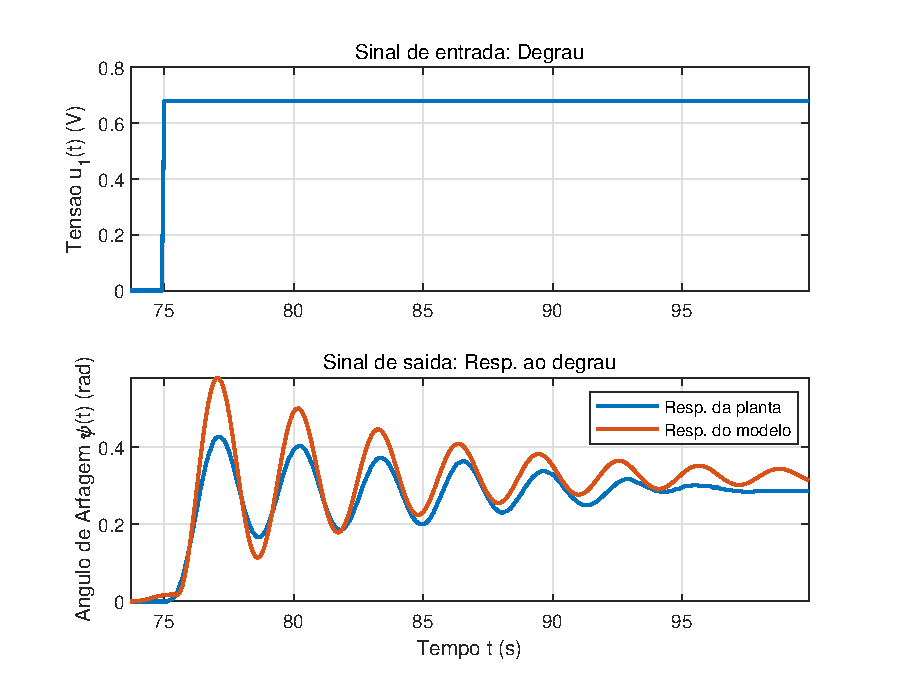
\includegraphics[width=0.45\textwidth]{figures/Validacao/ValidaPitchDegrau.eps}
    \caption{\textit{Pitch}: Sinal de entrada em degrau e resposta da planta e do modelo a essa entrada.}
    \label{fig:ValidaPitchDegrau}
\end{figure}

Já a Figura \ref{fig:ValidaPitchSenoide} mostra a resposta a uma entrada senoidal de amplitude $\SI{0.34}{\volt}$ e frequência $\SI{0.1}{\Hz}$.

\begin{figure}[H]
    \centering
    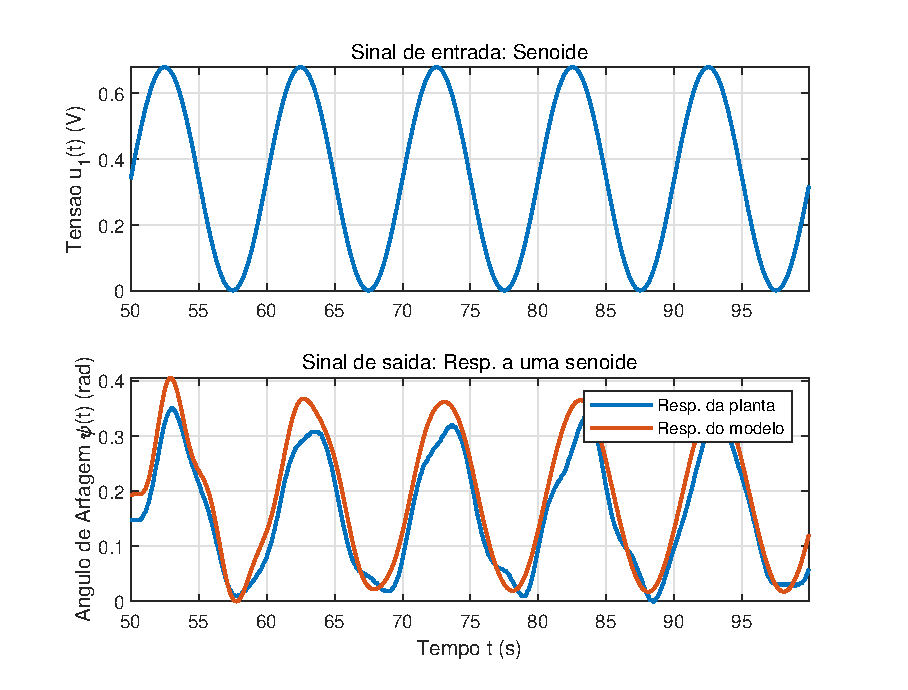
\includegraphics[width=0.45\textwidth]{figures/Validacao/ValidaPitchSenoide.eps}
    \caption{\textit{Pitch}: Sinal de entrada senoidal e resposta da planta e do modelo a essa entrada.}
    \label{fig:ValidaPitchSenoide}
\end{figure}

Pode-se observar pelas respostas obtidas que o modelo se aproxima de forma satisfatória do comportamento da planta, com amplitude, frequência de oscilação e amortecimentos próximos.

%%%%%%%%%%%%%%%%%%%%%%%%%%%%%%%%%%%%%%%%%%%%%%%%%%%%%%%%%%%%%%%%%%%
\subsection{\textbf{Validação do Modelo do \textit{yaw}}}

O modelo obtido para o ângulo \textit{yaw} foi validado também para sinais de entrada do tipo pulso e senoide. Os quais são mostrados nas Figuras \ref{fig:ValidaYawPulso} e \ref{fig:ValidaYawSenoide}.

Na Figura \ref{fig:ValidaYawPulso}, aplicou-se um pulso de amplitude $\SI{0.6}{\volt}$, com período de $T = \SI{50}{\s}$.

\begin{figure}[H]
    \centering
    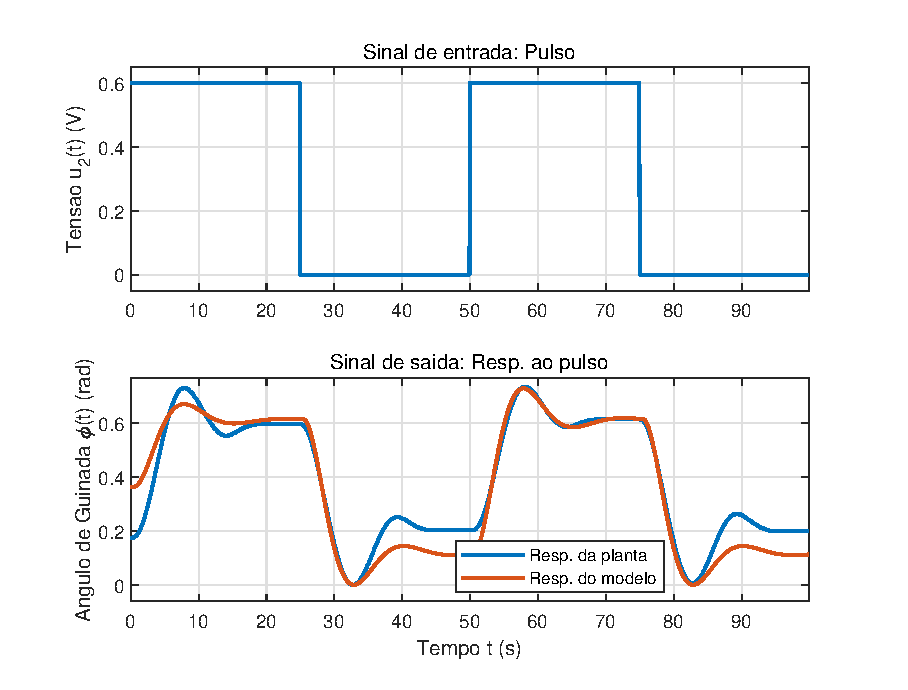
\includegraphics[width=0.48\textwidth]{figures/Validacao/ValidaYawPulso.eps}
    \caption{\textit{Yaw}: Sinal de entrada em pulso e resposta da planta e do modelo a essa entrada.}
    \label{fig:ValidaYawPulso}
\end{figure}

Pode-se observar que o modelo foi capaz de modelar corretamente o comportamento do ângulo de guinada, principalmente em se tratando de degraus positivos, nos quais tanto a amplitude quanto o amortecimento e a frequência ficaram bem ajustados.

Na Figura \ref{fig:ValidaYawSenoide}, o modelo para o \textit{yaw} é validado para uma entrada senoidal de amplitude $\pm \SI{0.3}{\volt}$, com período de $T = \SI{20}{\s}$.

\begin{figure}[H]
    \centering
    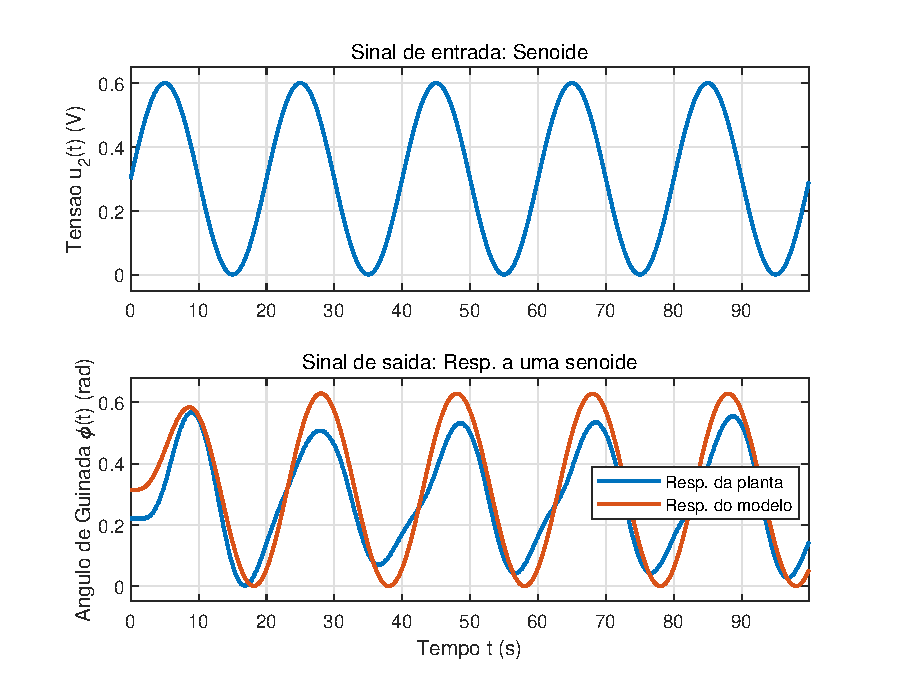
\includegraphics[width=0.48\textwidth]{figures/Validacao/ValidaYawSenoide.eps}
    \caption{\textit{Yaw}: Sinal de entrada senoidal e resposta da planta e do modelo a essa entrada.}
    \label{fig:ValidaYawSenoide}
\end{figure}

Observa-se que o modelo seguiu o comportamento original da planta, em termos de frequência de oscilação, destoando um pouco apenas na amplitude.

%%%%%%%%%%%%%%%%%%%%%%%%%%%%%%%%%%%%%%%%%%%%%%%%%%%%%%%%%%%%%%%%%%%
\subsection{\textbf{Validação do Modelo do \textit{cross-pitch}}}

A validação do modelo obtido para o \textit{cross-pitch} para sinais de entrada do tipo pulso e senoide, são apresentados nas Figuras \ref{fig:ValidaCrossPitchPulso} e \ref{fig:ValidaCrossPitchSenoide}.

Na Figura \ref{fig:ValidaCrossPitchPulso}, foi aplicado um pulso de amplitude $\pm \SI{0.5}{\volt}$, com frequência de $f = 1/\SI{50}{\s} = \SI{0.02}{\Hz}$.

\begin{figure}[H]
    \centering
    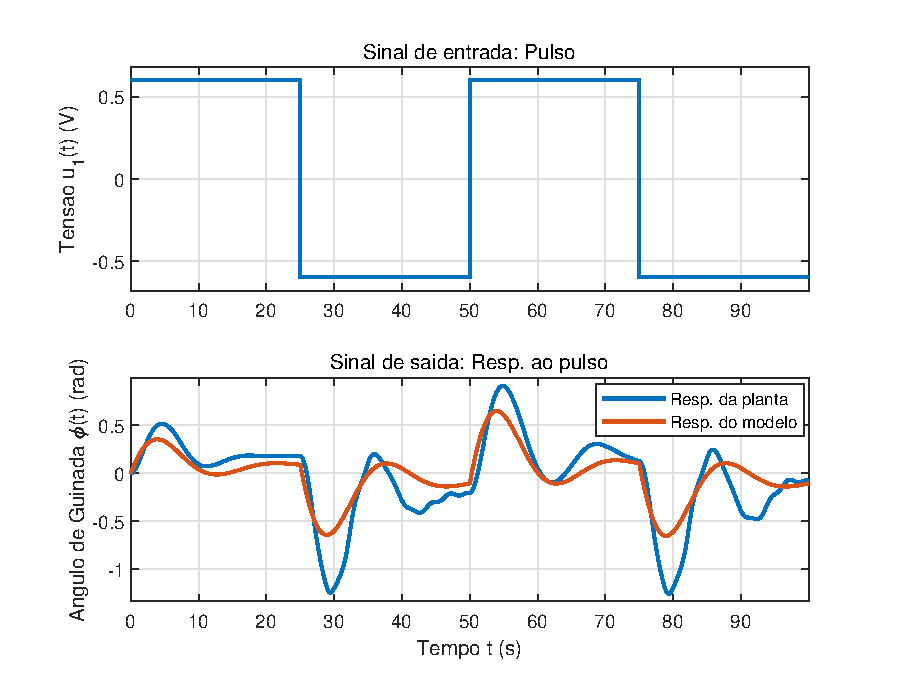
\includegraphics[width=0.48\textwidth]{figures/Validacao/ValidaCrossPitchPulso.eps}
    \caption{\textit{Cross-pitch}: Sinal de entrada em pulso e resposta da planta e do modelo a essa entrada.}
    \label{fig:ValidaCrossPitchPulso}
\end{figure}

Para amplitudes positivas, o modelo se aproximou melhor do comportamento real do sinal. 

Na Figura \ref{fig:ValidaCrossPitchSenoide}, foi aplicado um sinal senoidal de amplitude $\pm \SI{0.3}{\volt}$, com período de $T = \SI{50}{\s}$.

\begin{figure}[H]
    \centering
    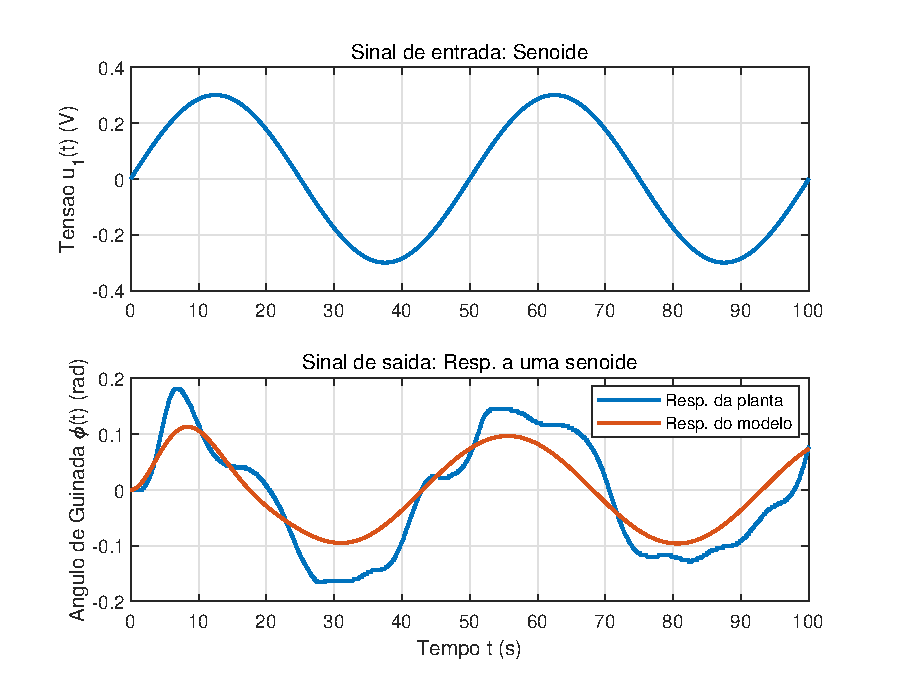
\includegraphics[width=0.48\textwidth]{figures/Validacao/ValidaCrossPitchSenoide.eps}
    \caption{\textit{Cross-pitch}: Sinal de entrada senoidal e resposta da planta e do modelo a essa entrada.}
    \label{fig:ValidaCrossPitchSenoide}
\end{figure}

Apesar das oscilações apresentadas pelo sinal original da planta, observa-se que o modelo foi capaz de seguir de forma razoável a trajetória correta.

%%%%%%%%%%%%%%%%%%%%%%%%%%%%%%%%%%%%%%%%%%%%%%%%%%%%%%%%%%%%%%%%%%%
\subsection{\textbf{Validação do Modelo do \textit{cross-yaw}}}

Na Figura \ref{fig:ValidaCrossYawPulso} é mostrada a resposta original da planta e a resposta do modelo para uma entrada em pulso com amplitude $\pm \SI{0.4}{\volt}$.

\begin{figure}[H]
    \centering
    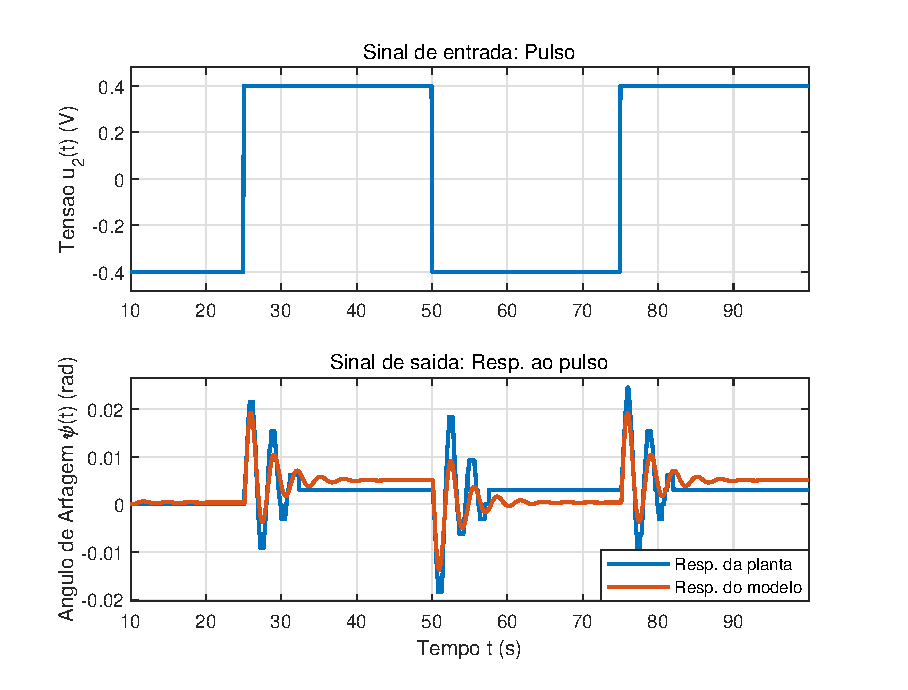
\includegraphics[width=0.48\textwidth]{figures/Validacao/ValidaCrossYawPulso.eps}
    \caption{\textit{Cross-yaw}: Sinal de entrada em pulso e resposta da planta e do modelo a essa entrada.}
    \label{fig:ValidaCrossYawPulso}
\end{figure}

Devido a baixa amplitude da resposta, da ordem de $\SI{e-3}{}$, e a impossibilidade de se aumentar a amplitude do sinal de entrada, devido a excursão limitada do giro do rotor, outros sinais de entrada não foram testados. Além disso, o período de amostragem, de $T_{s} = \SI{0.001}{\s}$, não pode ser reduzido ainda mais para se obter melhores resoluções, pois ao fazer isso, a quantidade de pontos de simulação era drasticamente reduzida.